\documentclass[aspectratio=169,10pt]{beamer}

\usepackage[utf8]{inputenc}
\usepackage[T1]{fontenc}
\usepackage[spanish]{babel}
\usepackage{lmodern}
\usepackage{graphicx}
\usepackage{booktabs}
\usepackage{tabularx}
\usepackage{array}
\usepackage{adjustbox}
\usepackage{xcolor}
\usepackage{amsmath}

\definecolor{santander}{HTML}{EC0000}
\definecolor{burgundy}{HTML}{8A1538}
\definecolor{darktext}{HTML}{2B2B2B}
\definecolor{softred}{HTML}{FBE7E7}
\definecolor{softgray}{HTML}{F4F4F4}
\definecolor{softgold}{HTML}{FFF2CC}
\definecolor{softteal}{HTML}{E6F2F1}
\definecolor{steelblue}{HTML}{1F77B4}
\definecolor{gold}{HTML}{C99700}
\definecolor{teal}{HTML}{007C7C}

\usetheme{Boadilla}
\usecolortheme{default}
\setbeamertemplate{navigation symbols}{}
\setbeamertemplate{footline}[frame number]
\setbeamercolor{frametitle}{fg=white,bg=burgundy}
\setbeamercolor{block title}{fg=white,bg=burgundy}
\setbeamercolor{block body}{fg=darktext,bg=softgray}
\setbeamercolor{alertblock title}{fg=white,bg=santander}
\setbeamercolor{alertblock body}{fg=darktext,bg=softred}
\setbeamercolor{normal text}{fg=darktext}
\setbeamerfont{frametitle}{series=\bfseries,size=\large}
\setlength{\tabcolsep}{3.5pt}
\renewcommand{\arraystretch}{1.10}
\setbeamersize{text margin left=6mm,text margin right=6mm}

\newcommand{\kpi}[3]{%
\begin{beamercolorbox}[wd=\linewidth,rounded=true,sep=4.5pt]{block body}
{\scriptsize\textcolor{burgundy}{\textbf{#1}}}\par
{\large\textbf{#2}}\par
{\scriptsize #3}
\end{beamercolorbox}}

\begin{document}

% Slide 1
\begin{frame}[t]{BRENT Pattern System - resumen ejecutivo}
\vspace{-0.10cm}
{\small Bundle multiactivo, ventanas de 32 días y EfficientNet-B1 para clasificación de patrones chartistas y regresión de retorno/niveles. Corte de datos: \textbf{2026-03-06}.}
\vspace{0.12cm}
\begin{columns}[T,onlytextwidth]
\begin{column}{0.34\textwidth}
\scriptsize
\begin{tabularx}{\linewidth}{>{\bfseries}p{0.43\linewidth}X}
\toprule
Activo & BRENT \\
Periodo base & 2007-01-02 a 2026-03-06 \\
Variables & 180 \\
Ventana & 32 días \\
Imagen & 160 $\times$ 160 RGB \\
Split & temporal, sin barajar \\
\bottomrule
\end{tabularx}
\vspace{0.12cm}
\begin{alertblock}{Punto crítico}
\scriptsize La corrida usa CPU y 1+1 épocas. La mejora inmediata es reentrenar en GPU de Colab con más épocas y misma partición temporal.
\end{alertblock}
\end{column}
\begin{column}{0.64\textwidth}
\begin{columns}[T,onlytextwidth]
\begin{column}{0.24\textwidth}\kpi{Exactitud test}{53.3\%}{Patrón principal}\end{column}
\begin{column}{0.24\textwidth}\kpi{Top-2 test}{81.6\%}{Clase correcta entre dos}\end{column}
\begin{column}{0.24\textwidth}\kpi{MAE retorno}{2.64 pp}{Horizonte 1 día}\end{column}
\begin{column}{0.24\textwidth}\kpi{Última señal}{+0.99\%}{asc. channel, p=84.2\%}\end{column}
\end{columns}
\vspace{0.18cm}
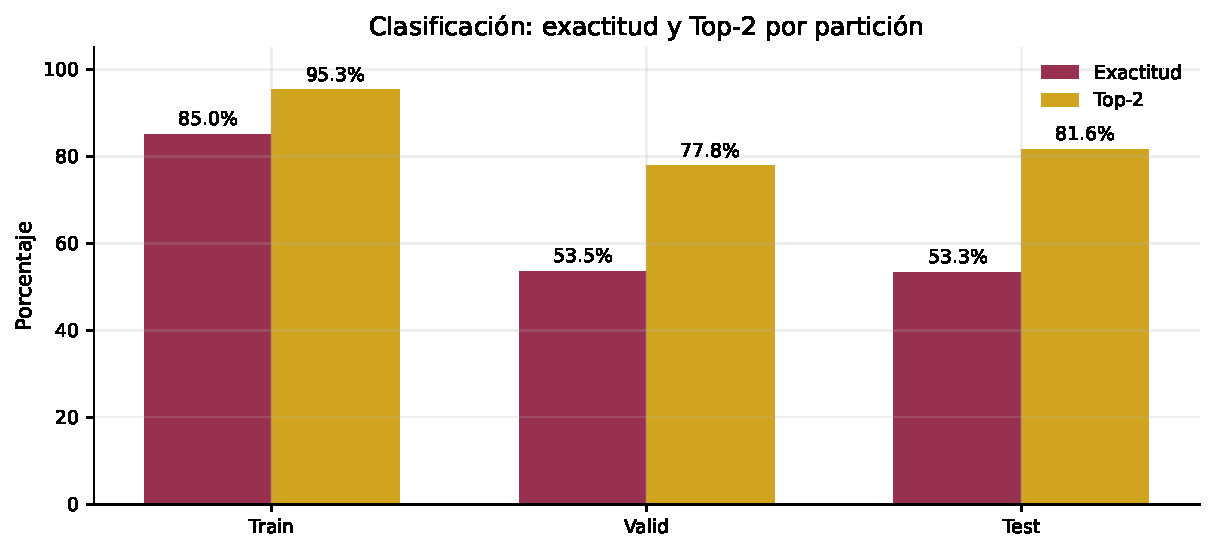
\includegraphics[width=\linewidth,height=0.41\textheight,keepaspectratio]{figures/metrics_by_split.pdf}
\end{column}
\end{columns}
\end{frame}

% Slide 2
\begin{frame}[t]{Inputs y partición temporal}
\begin{center}
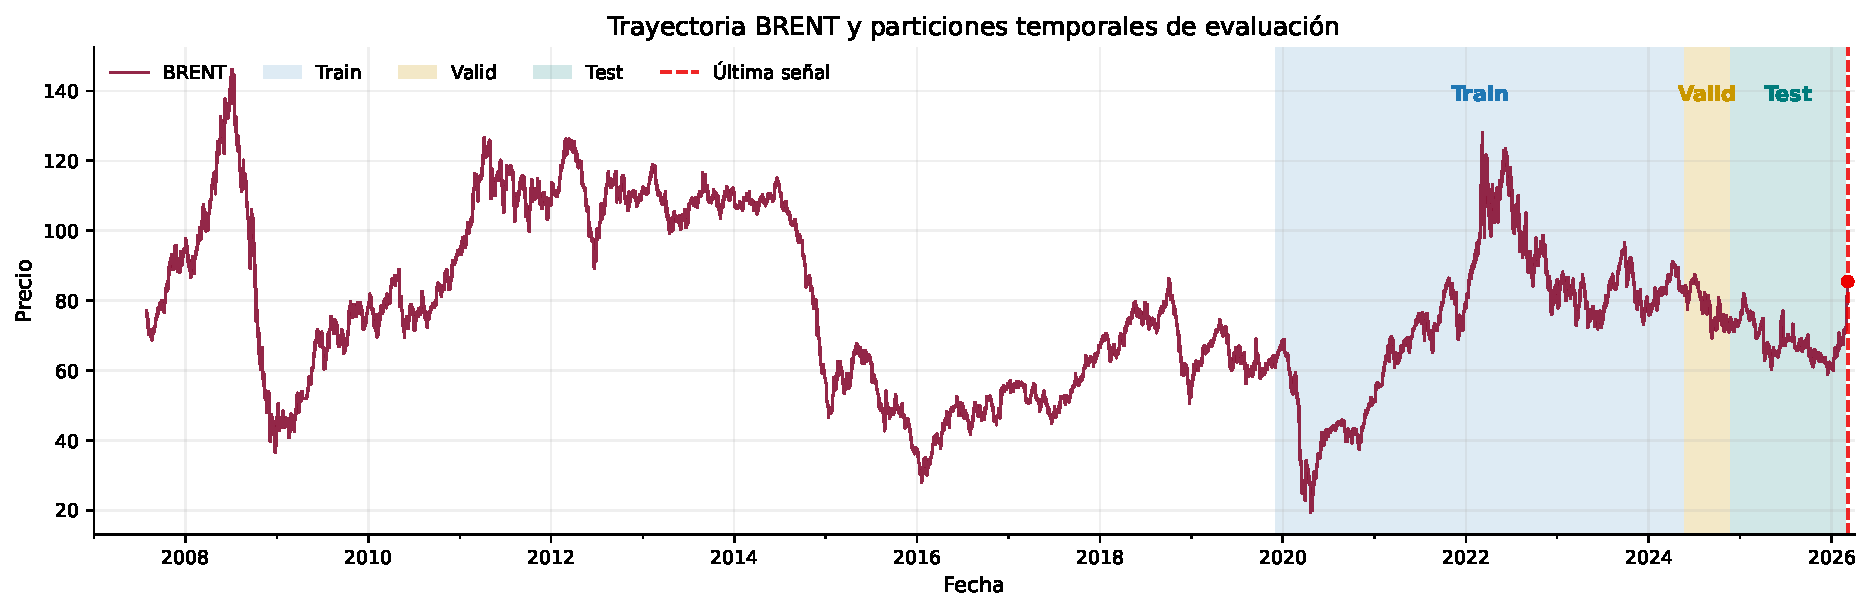
\includegraphics[width=0.96\linewidth,height=0.52\textheight,keepaspectratio]{figures/timeline_splits.pdf}
\end{center}
\vspace{-0.16cm}
\begin{columns}[T,onlytextwidth]
\begin{column}{0.53\textwidth}
\scriptsize
\begin{tabularx}{\linewidth}{lrrr}
\toprule
Partición & Ventanas & Inicio & Fin \\
\midrule
Train etiquetado & 887 & 2019-12-02 & 2024-05-21 \\
Validación & 99 & 2024-05-22 & 2024-11-20 \\
Test etiquetado & 244 & 2024-11-21 & 2026-02-26 \\
\midrule
Tensor train & 986 & 2019-12-02 & 2024-11-20 \\
Tensor test & 247 & 2024-11-21 & 2026-03-04 \\
\bottomrule
\end{tabularx}
\end{column}
\begin{column}{0.45\textwidth}
\scriptsize
\begin{tabularx}{\linewidth}{>{\bfseries}p{0.42\linewidth}X}
\toprule
Fuentes & Yahoo Finance, FRED, BCE AAA \\
Series base & 37 \\
Target & \texttt{BRENT\_fwd\_logret\_1} \\
Horizonte & 1 día \\
Normalización & media/desv. de train \\
\bottomrule
\end{tabularx}
\end{column}
\end{columns}
\end{frame}

% Slide 3
\begin{frame}[t]{Metodología del experimento}
\begin{columns}[T,onlytextwidth]
\begin{column}{0.53\textwidth}
\small
\begin{block}{Flujo académico}
\begin{enumerate}\setlength\itemsep{0.20em}
\item Descarga y alineación diaria de series de mercado.
\item Matriz \emph{wide}: precios, retornos, volatilidad, rangos, medias, spreads y ratios.
\item Estandarización con estadísticos de train.
\item Ventanas 32 $\times$ 180 y codificación RGB.
\item Evaluación con train, validación y hold-out temporal.
\end{enumerate}
\end{block}
\vspace{0.06cm}
\begin{alertblock}{Criterio de evaluación}
\scriptsize El tramo de test es posterior al entrenamiento; no hay mezcla aleatoria de fechas entre particiones.
\end{alertblock}
\end{column}
\begin{column}{0.45\textwidth}
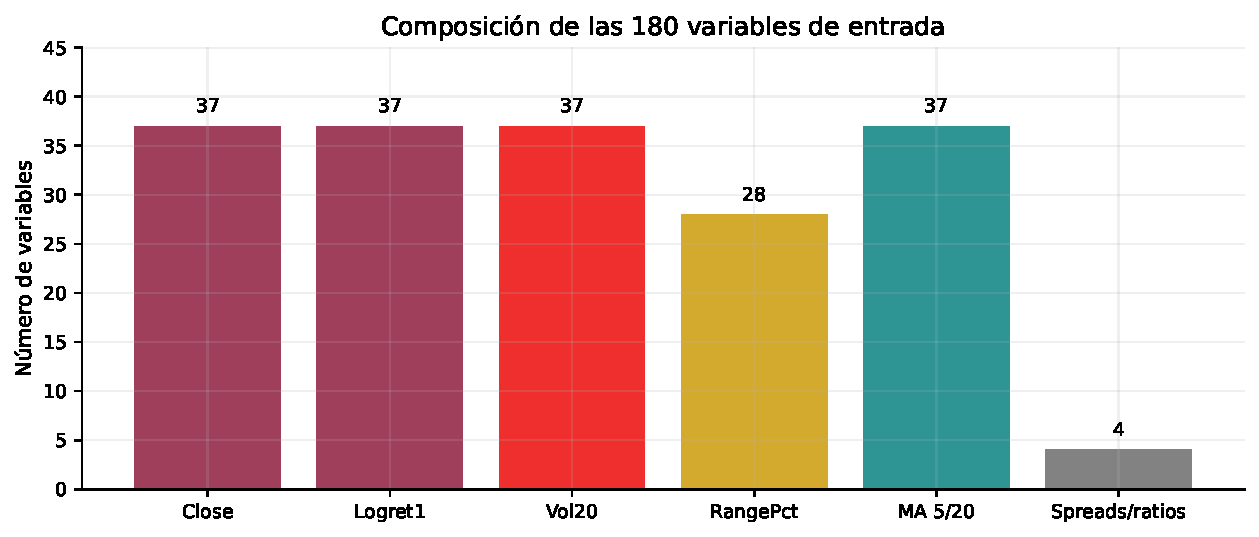
\includegraphics[width=\linewidth,height=0.43\textheight,keepaspectratio]{figures/feature_groups_compact.pdf}
\vspace{0.05cm}
\scriptsize
\begin{tabularx}{\linewidth}{>{\bfseries}p{0.41\linewidth}X}
\toprule
Modelo & EfficientNet-B1 multitarea \\
Salidas & patrón, retorno, low, high \\
Regresión loss & peso 0.5 \\
Batch size & 8 \\
Entrenamiento & CPU, 1 + 1 épocas \\
\bottomrule
\end{tabularx}
\end{column}
\end{columns}
\end{frame}

% Slide 4
\begin{frame}[t]{Resultados principales en test}
\begin{columns}[T,onlytextwidth]
\begin{column}{0.49\textwidth}
\centering
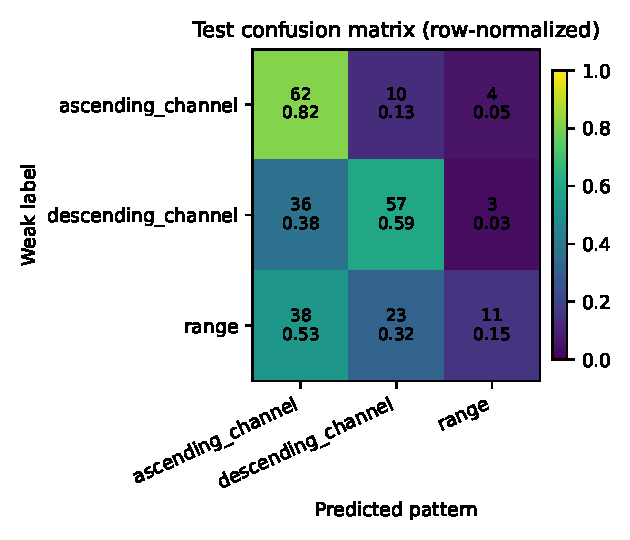
\includegraphics[width=0.92\linewidth,height=0.52\textheight,keepaspectratio]{figures/test_confusion_matrix.pdf}
\end{column}
\begin{column}{0.49\textwidth}
\centering
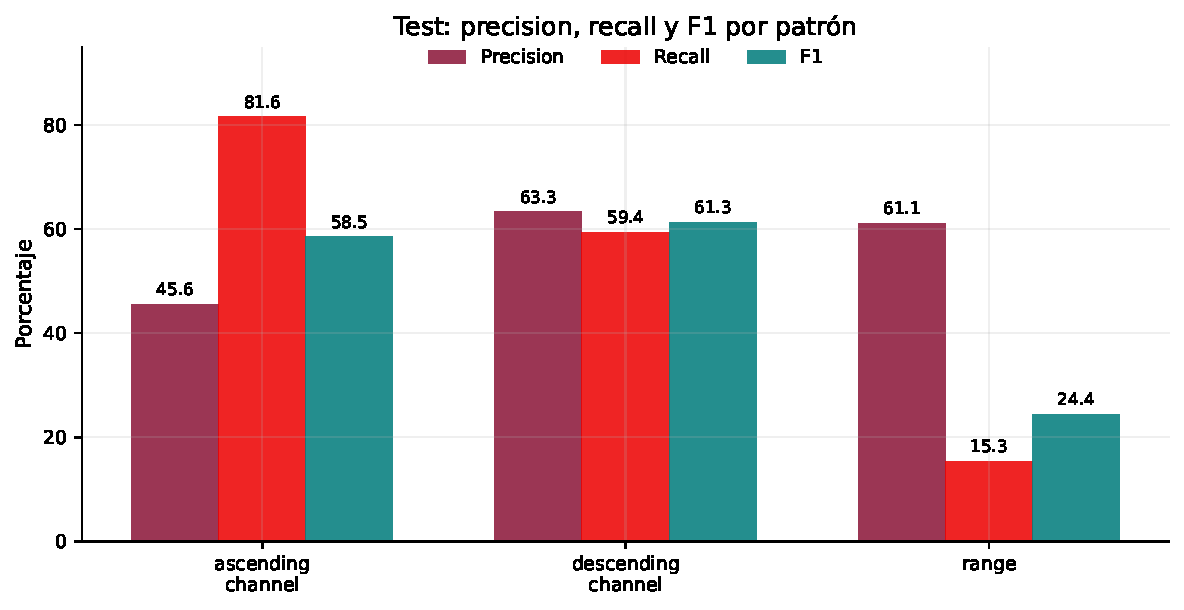
\includegraphics[width=\linewidth,height=0.46\textheight,keepaspectratio]{figures/test_prf_bars.pdf}
\end{column}
\end{columns}
\vspace{-0.08cm}
\begin{columns}[T,onlytextwidth]
\begin{column}{0.54\textwidth}
\scriptsize
\begin{tabularx}{\linewidth}{lrrrr}
\toprule
Clase & Prec. & Recall & F1 & Soporte \\
\midrule
\texttt{ascending\_channel} & 45.6\% & 81.6\% & 58.5\% & 76 \\
\texttt{descending\_channel} & 63.3\% & 59.4\% & 61.3\% & 96 \\
\texttt{range} & 61.1\% & 15.3\% & 24.4\% & 72 \\
\bottomrule
\end{tabularx}
\end{column}
\begin{column}{0.44\textwidth}
\scriptsize
\begin{tabularx}{\linewidth}{>{\bfseries}p{0.48\linewidth}X}
\toprule
Exactitud & 53.3\% \\
Top-2 & 81.6\% \\
MAE retorno & 2.64 pp \\
RMSE retorno & 3.40 pp \\
Acierto signo & 52.46\% \\
\bottomrule
\end{tabularx}
\end{column}
\end{columns}
\end{frame}

% Slide 5
\begin{frame}[t]{Siguientes pasos de mejora}
\vspace{-0.05cm}
\begin{beamercolorbox}[wd=\linewidth,rounded=true,sep=5pt]{block body}
\small \textbf{Última señal:} \texttt{ascending\_channel}, probabilidad 84.2\%, retorno esperado +0.987\%, \texttt{outlier\_flag=1}. La prioridad es mejorar el entrenamiento antes de interpretar la señal como estable.
\end{beamercolorbox}
\vspace{0.12cm}
\begin{columns}[T,onlytextwidth]
\begin{column}{0.43\textwidth}
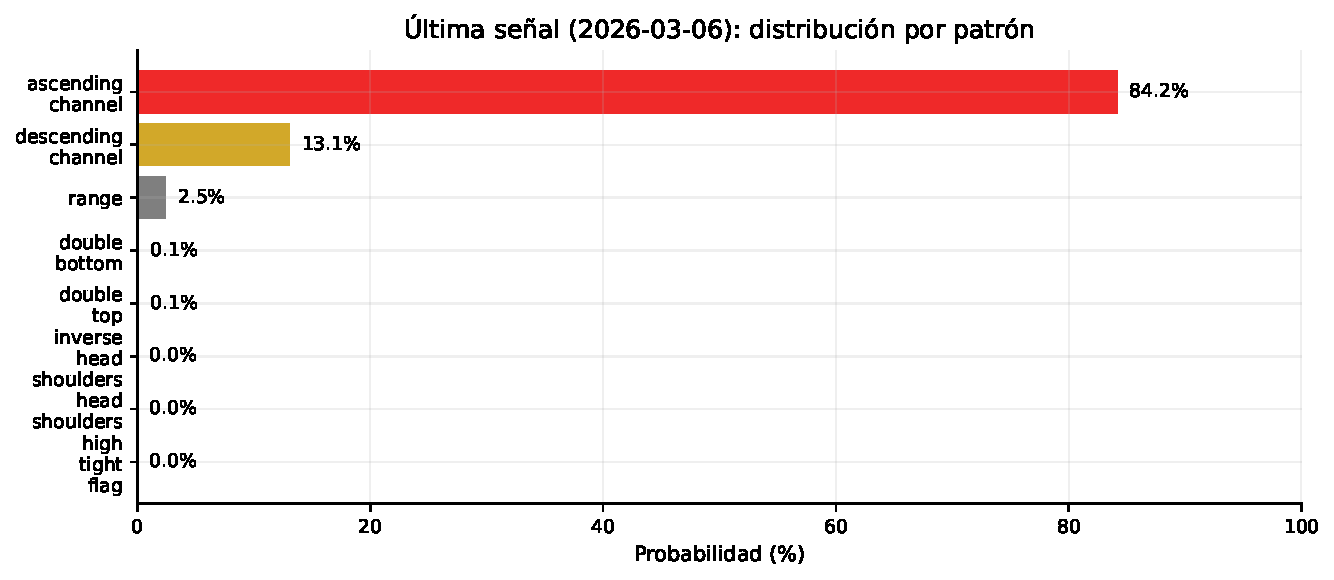
\includegraphics[width=\linewidth,height=0.43\textheight,keepaspectratio]{figures/latest_probabilities.pdf}
\vspace{0.06cm}
\begin{alertblock}{Brecha operativa}
\scriptsize \texttt{device=cpu}, \texttt{pretrained\_backbone=false}, \texttt{use\_synthetic\_pretrain=false}, 1+1 épocas.
\end{alertblock}
\end{column}
\begin{column}{0.55\textwidth}
\small
\begin{block}{Roadmap recomendado}
\begin{enumerate}\setlength\itemsep{0.25em}
\item \textbf{GPU Colab:} activar \texttt{device=cuda}, registrar CUDA y usar mixed precision.
\item \textbf{Entrenamiento:} ampliar épocas, early stopping y pruebas con backbone preentrenado.
\item \textbf{Validación:} walk-forward por regímenes de mercado y reporte por ventana temporal.
\item \textbf{Calibración:} probabilidades, umbrales de outlier y consistencia \texttt{low/high}.
\item \textbf{Ablación:} importancia de grupos de features y comparación contra baselines.
\end{enumerate}
\end{block}
\end{column}
\end{columns}
\end{frame}

\end{document}
